\section{Annexes: Diagrammes fonctionnels}

	\subsection{Module maître}
		
		\begin{figure}[H]
			\centering
			\fbox{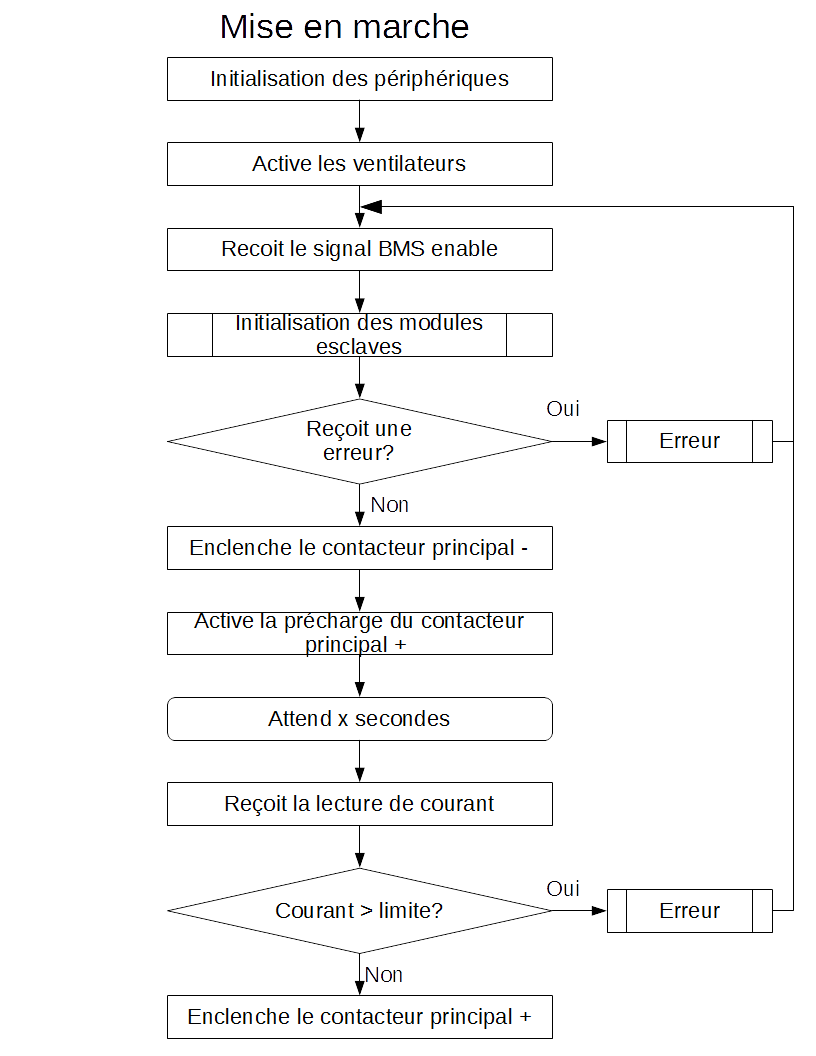
\includegraphics[width=0.5\linewidth]{Images/DiagrammeFonctionnel_MiseEnMarche}}
			\caption{Diagramme module maître: Mise en marche}
			\label{fig:diagrammefonctionnelmiseenmarche}
		\end{figure}
		
		\begin{figure}[H]
			\centering
			\fbox{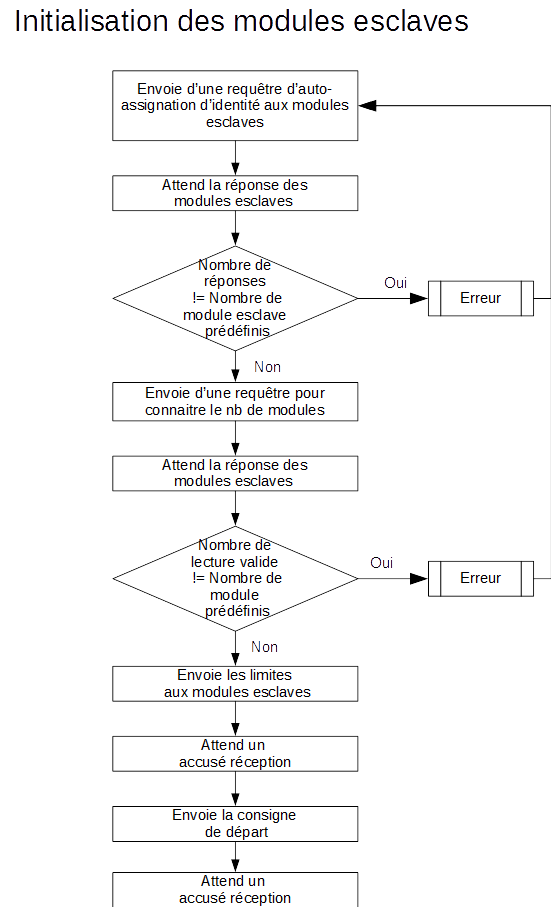
\includegraphics[width=0.7\linewidth]{Images/DiagrammeFonctionnel_MaitreInitEsclave}}
			\caption{Diagramme module maître: Initialisation des modules esclaves}
			\label{fig:diagrammefonctionnelmaitreinitesclave}
		\end{figure}
		
		\begin{figure}[H]
			\centering
			\fbox{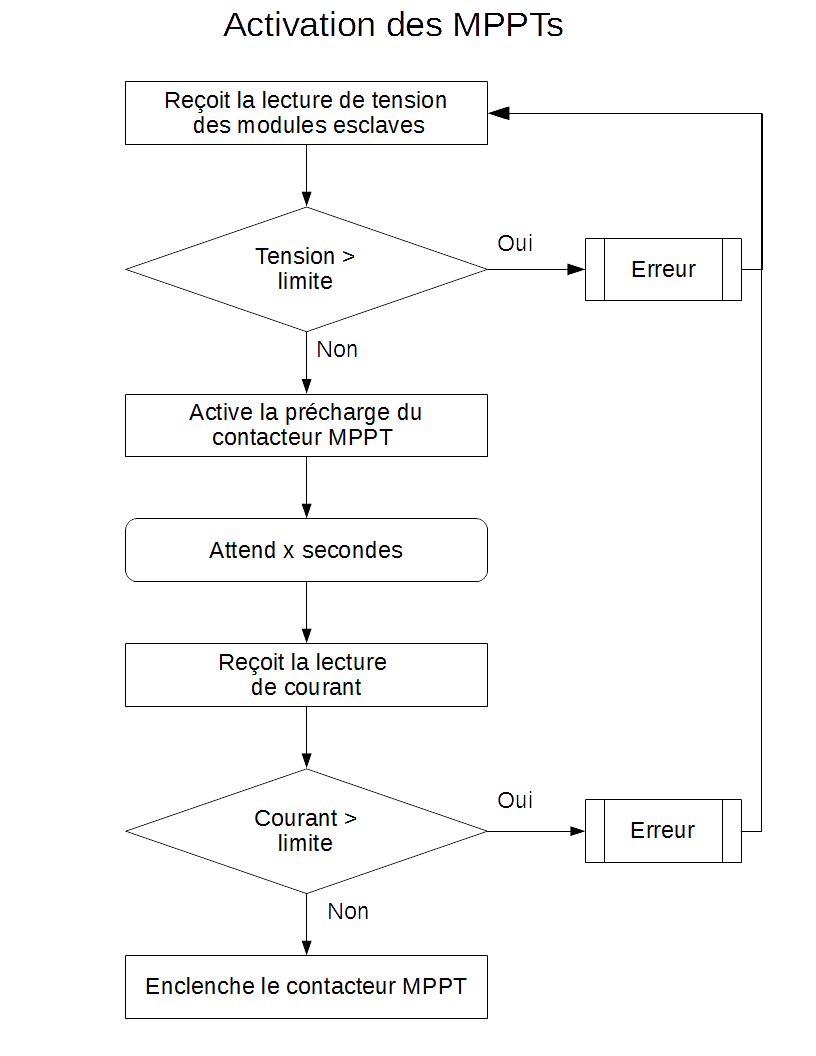
\includegraphics[width=0.7\linewidth]{Images/DiagrammeFonctionnel_ActivationMppt}}
			\caption{Diagramme module maître: Activation des MPPTs}
			\label{fig:diagrammefonctionnelactivationmppt}
		\end{figure}
		
		\begin{figure}[H]
			\centering
			\fbox{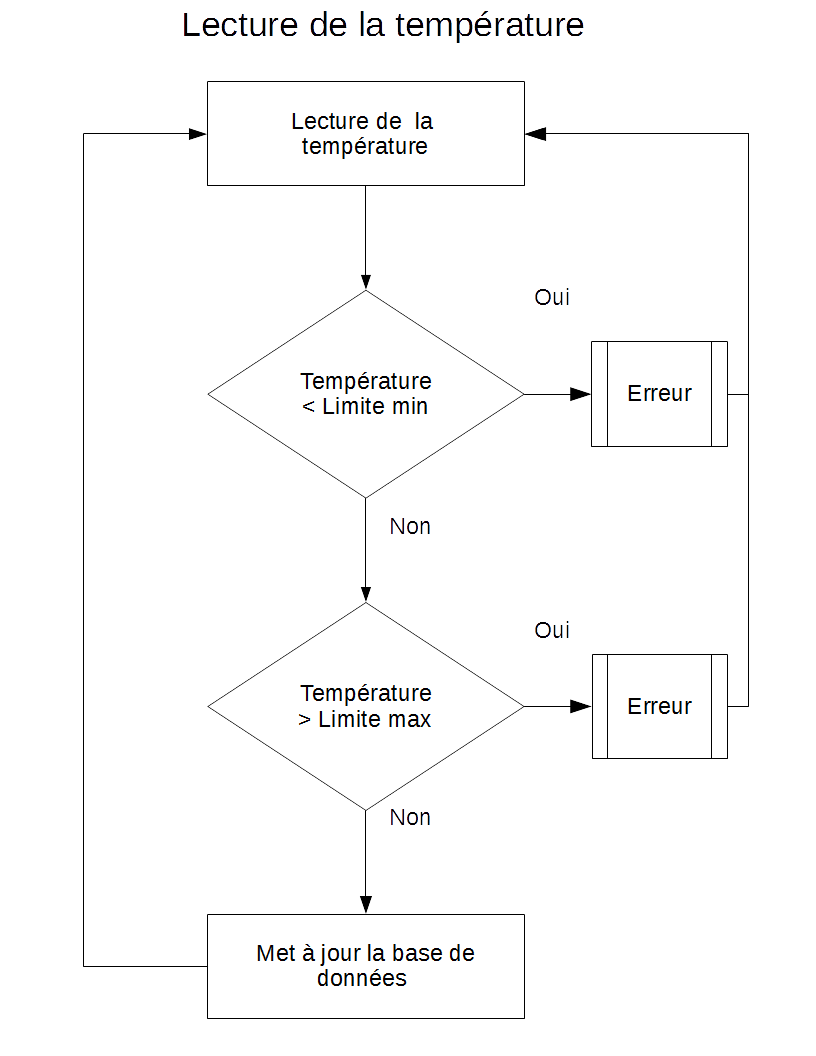
\includegraphics[width=0.7\linewidth]{Images/DiagrammeFonctionnel_MaitreLectureTemp}}
			\caption{Diagramme module maître: Lecture de la température}
			\label{fig:diagrammefonctionnelmaitrelecturetemp}
		\end{figure}
			
		\begin{figure}[H]
			\centering
			\fbox{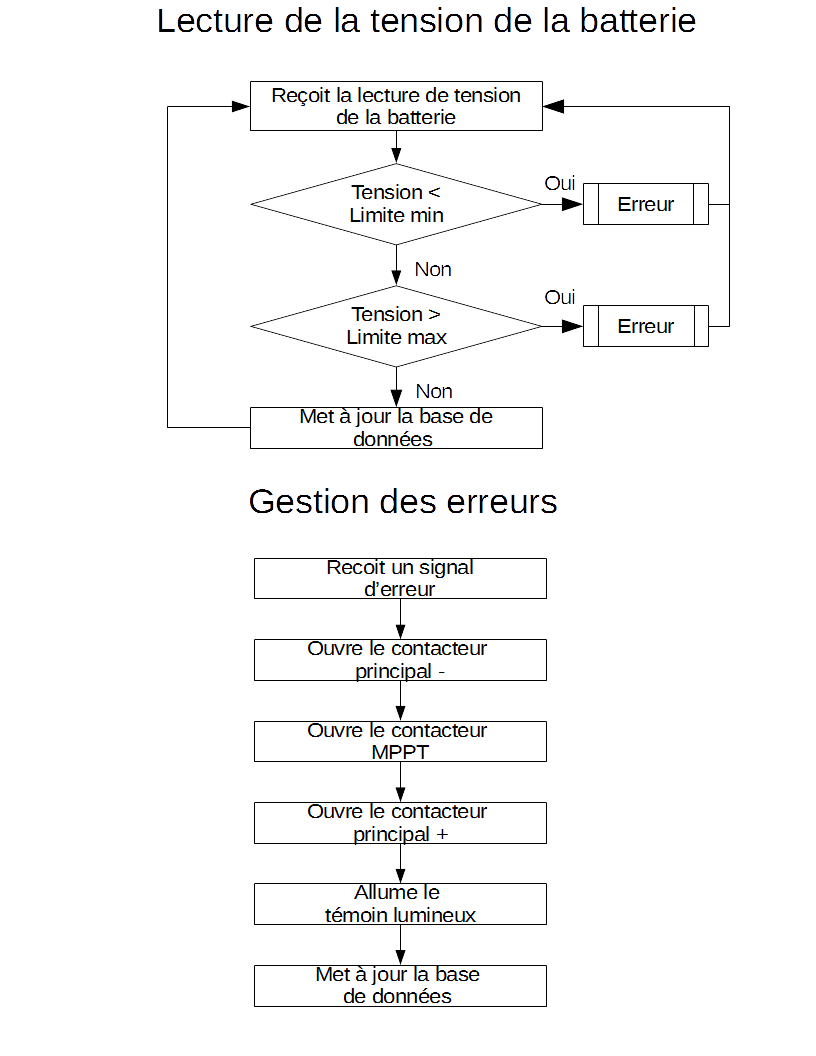
\includegraphics[width=0.7\linewidth]{Images/DiagrammeFonctionnel_MaitreLectureBat}}
			\caption{Diagramme module maître: Lecture de la tension de la batterie + Gestion des erreurs}
			\label{fig:diagrammefonctionnelmaitrelecturebat}
		\end{figure}
			
		\begin{figure}[H]
			\centering
			\fbox{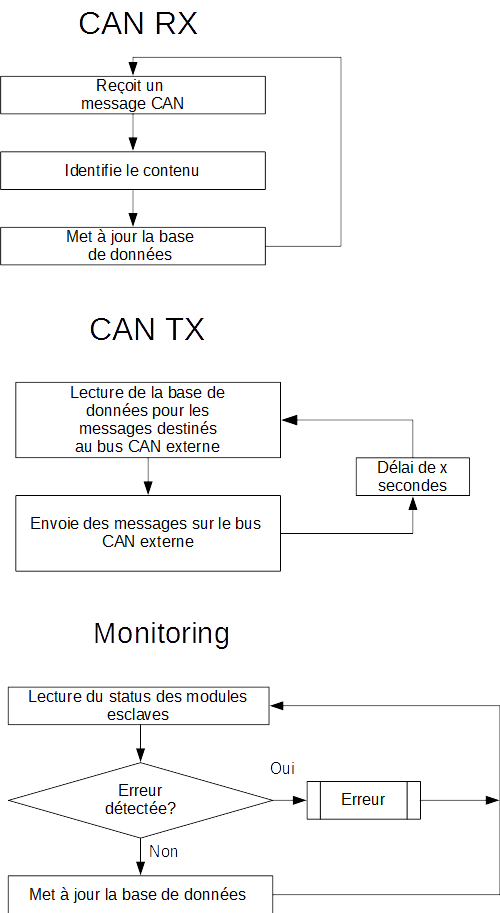
\includegraphics[width=0.7\linewidth]{Images/DiagrammeFonctionnel_CanMonitoring}}
			\caption{Diagramme module maître: CAN RX + CAN TX + Monitoring }
			\label{fig:diagrammefonctionnelcanmonitoring}
		\end{figure}
			
	\subsection{Module esclave}
	
		\begin{figure}[H]
			\centering
			\fbox{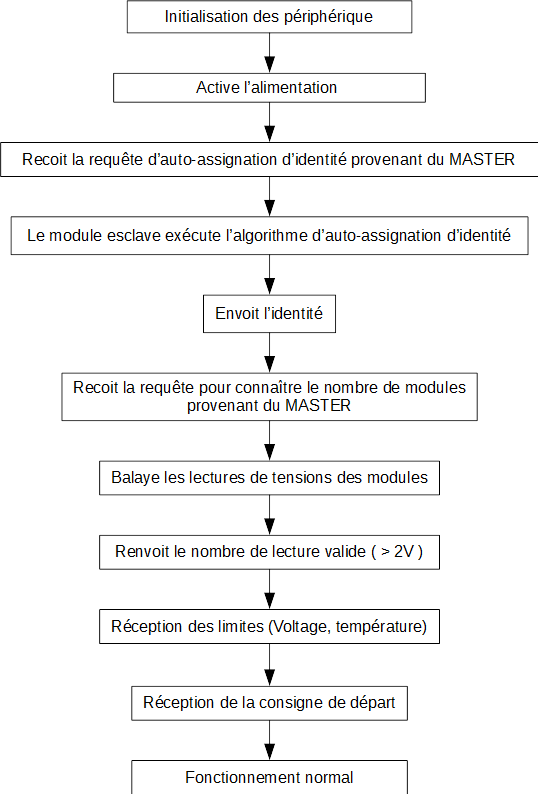
\includegraphics[width=0.7\linewidth]{Images/DiagrammeFonctionnel_SlaveMiseEnMarche}}
			\caption{Digramme module esclave: Mise en marche}
			\label{fig:diagrammefonctionnelslavemiseenmarche}
		\end{figure}
		
		\begin{figure}[H]
			\centering
			\fbox{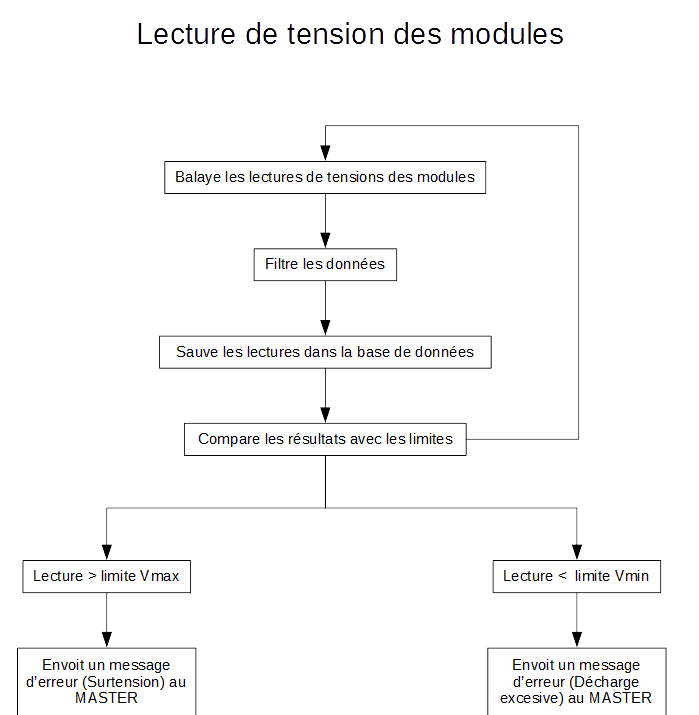
\includegraphics[width=0.7\linewidth]{Images/DiagrammeFonctionnel_SlaveLectureDeTension}}
			\caption{Diagramme module esclave: Lecture de tension des modules}
			\label{fig:diagrammefonctionnelslavelecturedetension}
		\end{figure}
		
		\begin{figure}[H]
			\centering
			\fbox{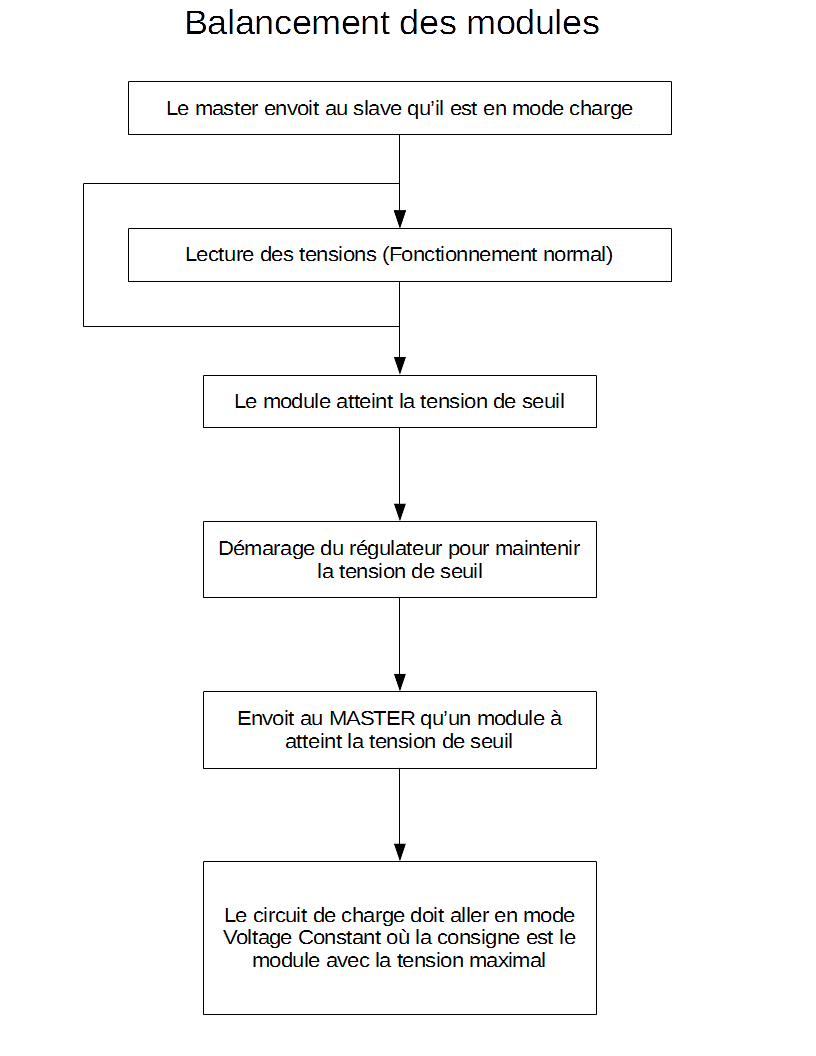
\includegraphics[width=0.7\linewidth]{Images/DiagrammeFonctionnel_SlaveBalancement}}
			\caption{Diagramme module esclave: Balancement des modules}
			\label{fig:diagrammefonctionnelslavebalancement}
		\end{figure}
	
		\begin{figure}[H]
			\centering
			\fbox{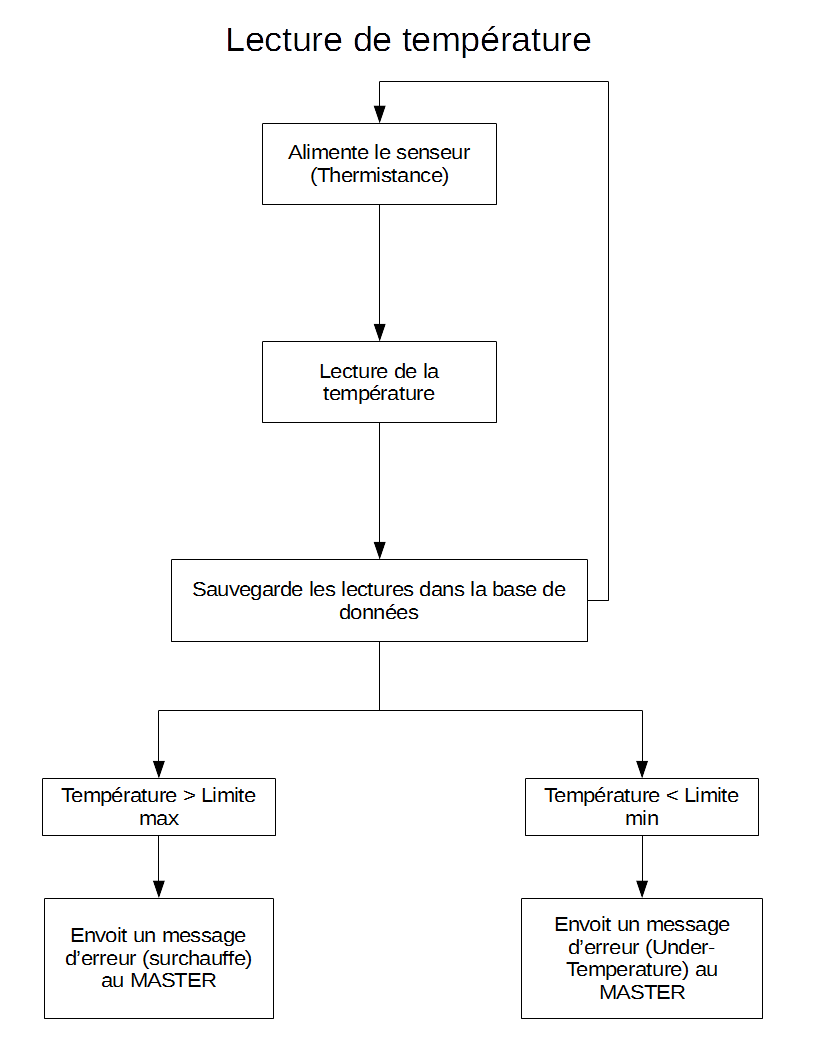
\includegraphics[width=0.7\linewidth]{Images/DiagrammeFonctionnel_SlaveLectureTemperature}}
			\caption{Diagramme module esclave: Lecture de température}
			\label{fig:diagrammefonctionnelslavelecturetemperature}
		\end{figure}

		\begin{figure}[H]
			\centering
			\fbox{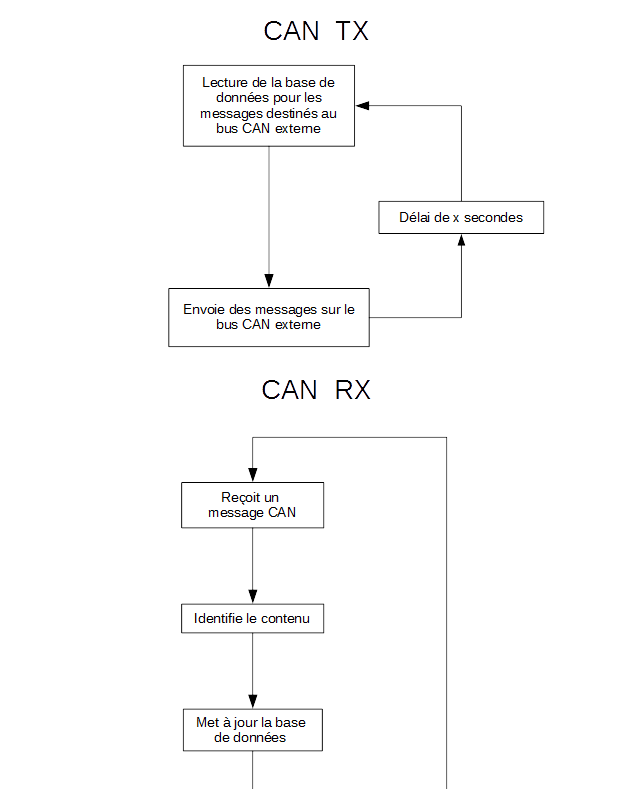
\includegraphics[width=0.7\linewidth]{Images/DiagrammeFonctionnel_SlaveCan}}
			\caption{Diagramme module esclave: CAN TX + CAN RX}
			\label{fig:diagrammefonctionnelslavecan}
		\end{figure}
		
	\subsection{Module de lecture de courant}

		\begin{figure}[H]
			\centering
			\fbox{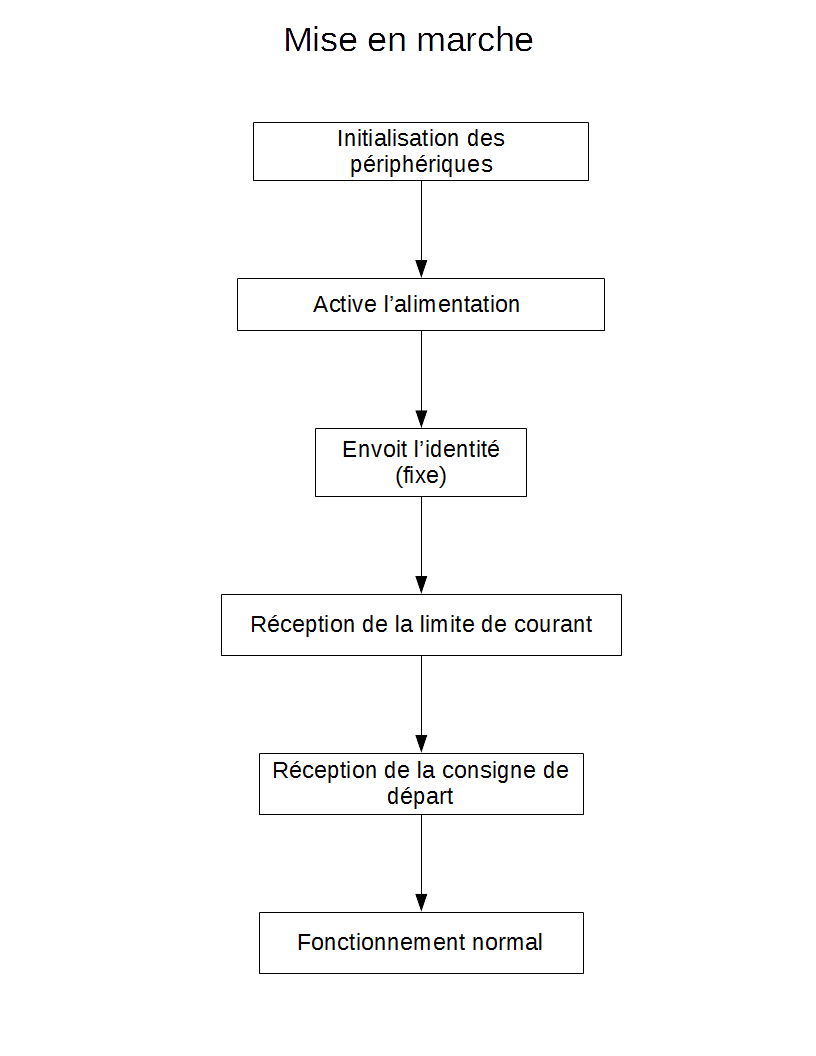
\includegraphics[width=0.7\linewidth]{Images/DiagrammeFonctionnel_CurrentMiseEnMarche}}
			\caption{Diagramme module de lecture de courant: Mise en marche}
			\label{fig:diagrammefonctionnelcurrentmiseenmarche}
		\end{figure}

		\begin{figure}[H]
			\centering
			\fbox{\includegraphics[width=0.7\linewidth]{"Images/DiagrammeFonctionnel_CurrentLecture de courant"}}
			\caption{Diagramme module de lecture de courant: Lecture de courant}
			\label{fig:diagrammefonctionnelcurrentlecture-de-courant}
		\end{figure}
				
		
		\begin{figure}[H]
			\centering
			\fbox{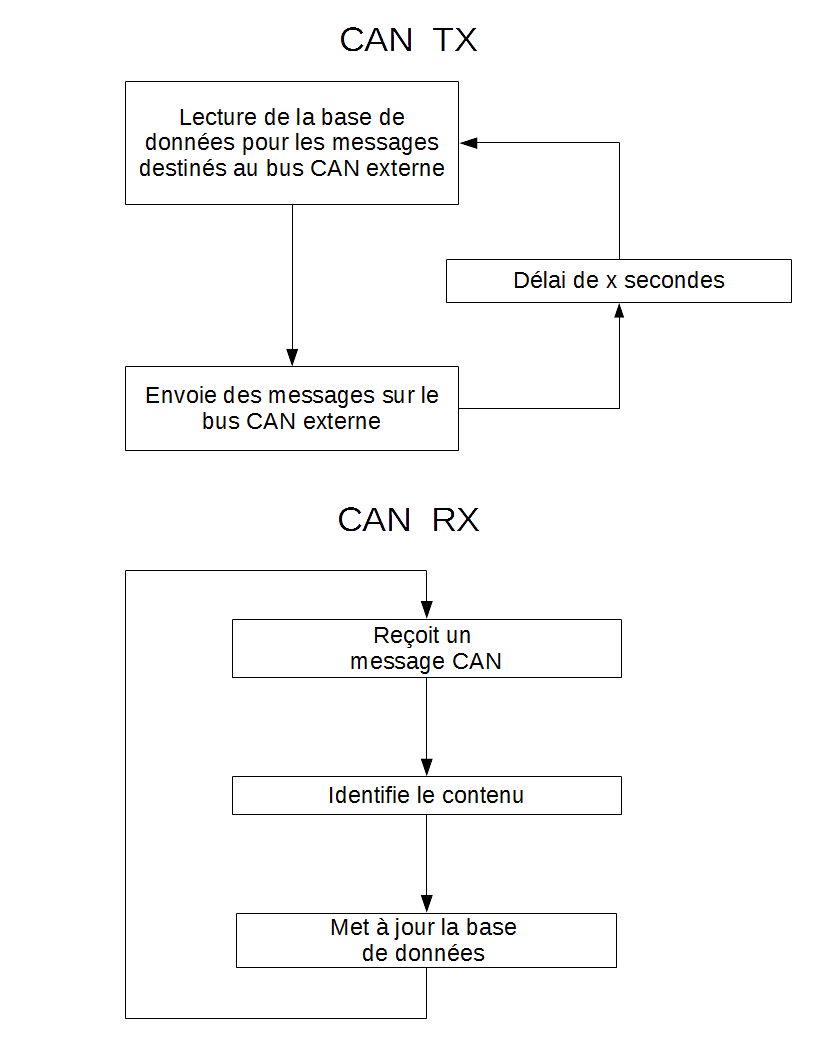
\includegraphics[width=0.7\linewidth]{Images/DiagrammeFonctionnel_CurrentCan}}
			\caption{Diagramme module de lecture de courant: CAN TX + CAN RX}
			\label{fig:diagrammefonctionnelcurrentcan}
		\end{figure}

\newpage